\subsection{Overview}
The high-level architecture of the system to be developed is illustrated below, which gives abstract information about different parts of the system. For the backend part, the system uses a VPS which is hosted on Hetzner company, renting VPS provides the possibility of avoiding problems related to managing server’s hardware and configuration. Furthermore, in order to guarantee the flexibility and scalability of the system for the future, we use \emph{Kubernetes} which is an open-source container-orchestration system, it allows us to maintain and manage containers in real-time. Moreover, to have a concrete development and deployment environment, we use \emph{Docker} containers that are also a proper method for implementing microservice architectures that will be elaborated in detail in the following sections. In this case, all services can operate independently. \\
What is more, for logging and error tracking both in frontend and backend, SafeStreet takes advantage of \emph{Sentry} which is a cloud-based monitoring application that allows us to prevent chaotic and inevitable errors in the SafeStreet system. Apart from this, \emph{Datadog} which is a monitoring service for cloud-scale applications is used for VPS monitoring, aiming to display relevant information of the VPS in real-time through a user-friendly and professional dashboard. \\
As a reliable geo-location service, the system uses the \emph{GoogleMap API} that provides rich functionality for our system. When it comes to security, the system utilizes \emph{Cloudflare’s} CDN, DNS/DNSSEC, Firewall, Rate limiting, Load balancing and SSL/TLS to ensure data confidentiality and integration. Additionally, for the aim of authentication and specialized database \emph{Firebase} is used, because of its simplicity that helps developers to implement their application. 


\begin{figure}[H]
\caption{High Level Architecture}
\label{fig:HighLevel}
\centering
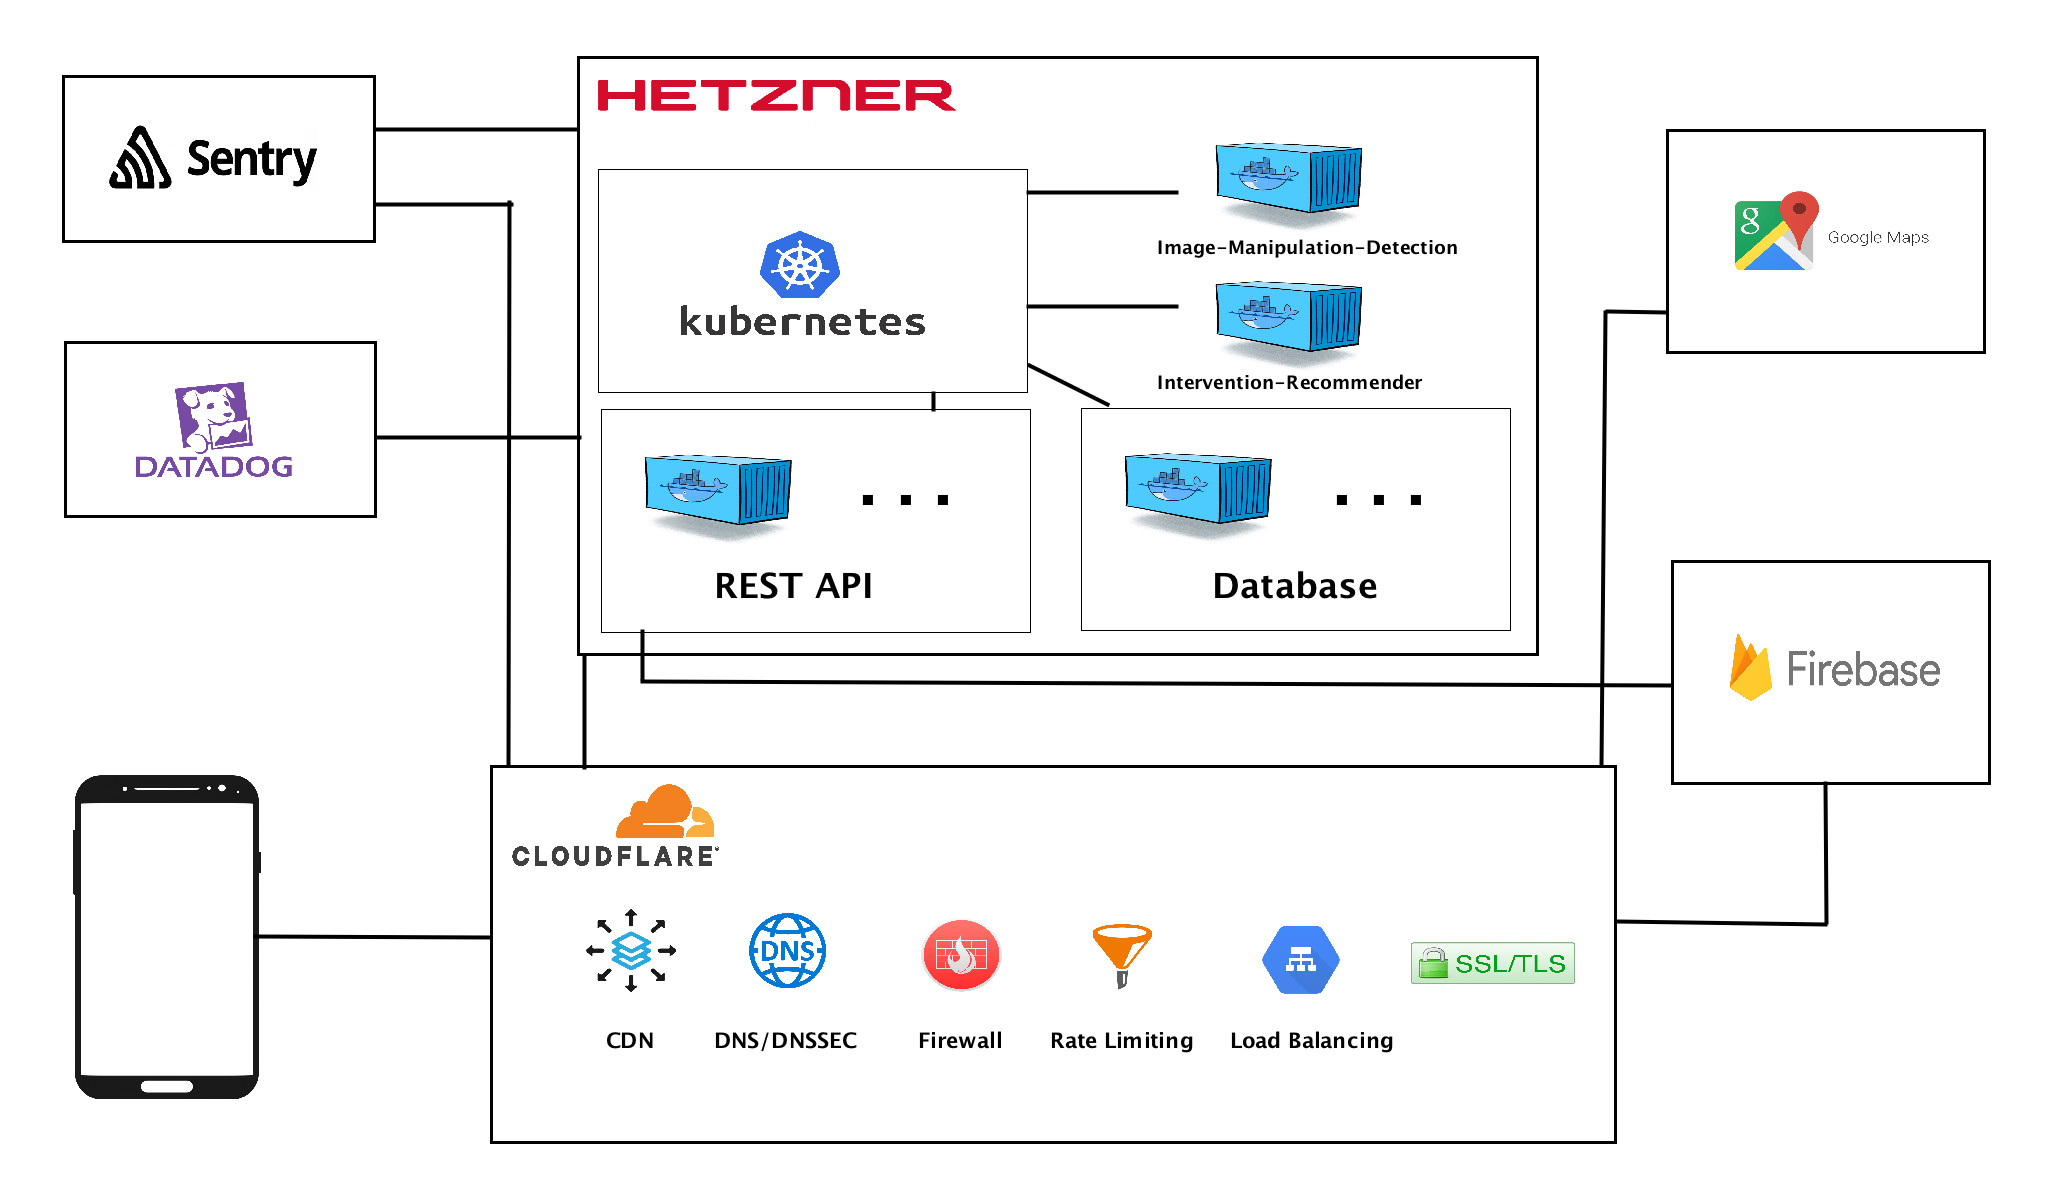
\includegraphics[width=\textwidth, height=0.5\textheight]{HighLevelDiagram.png}
\end{figure}
